\documentclass{beamer}

\usepackage[utf8]{inputenc}
\usepackage[T1]{fontenc}
\usepackage[french]{babel}
\usepackage[babel=true]{csquotes} % guillements français
\usepackage{graphicx}
\graphicspath{{Images/}{Images/L3_Android/}}
\usepackage{color}
\usepackage{hyperref}
\hypersetup{colorlinks,linkcolor=,urlcolor=blue}


\mode<presentation>
{
  %% PLUSIEURS THEMES EXISTENT : VOIR DOCUMENTATION
  % \usetheme{Warsaw}
  % \usetheme{Frankfurt}
  \usetheme{Madrid}
  % or ...

  \setbeamercovered{transparent}
  % or whatever (possibly just delete it)
}


\title[Dev. Mobiles -- L3 info]{Développement pour mobiles\\L3 Informatique\\\textbf{Jeu de dame}}
\author{Billy Ronico, Ismael Saïd}
\institute[DI]{Université de la Réunin}
\date{\today}


\subject{Talks}
% This is only inserted into the PDF information catalog. Can be left
% out.



% If you have a file called "university-logo-filename.xxx", where xxx
% is a graphic format that can be processed by latex or pdflatex,
% resp., then you can add a logo as follows:

% \pgfdeclareimage[height=0.5cm]{university-logo}{university-logo-filename}
% \logo{\pgfuseimage{university-logo}}



% Delete this, if you do not want the table of contents to pop up at
% the beginning of each subsection:
\AtBeginSection[]
{
  \begin{frame}<beamer>
    \frametitle{Plan}
    \tableofcontents[currentsection]
  \end{frame}
}

% \AtBeginSubsection[]
% {
%   \begin{frame}<beamer>
%     \frametitle{Plan}
%     \tableofcontents[currentsection,currentsubsection]
%   \end{frame}
% }


% If you wish to uncover everything in a step-wise fashion, uncomment
% the following command:

%\beamerdefaultoverlayspecification{<+->}


\begin{document}

\begin{frame}
  \titlepage
\end{frame}


%%%%%%%%%%%%%%%%%%%%
\section{Introduction}
%%%%%%%%%%%%%%%%%%%%
%
%
\begin{frame}
  \frametitle{Introduction}
    \subsection{Presentation du jeu de dame}
    Le jeu de dame est un jeu de strategie qui date du debut du 18 ème siècle. 
    
    Il se joue sur un damier de taille n * n (en général 10 * 10).

    L'objéctif du jeu est de prendre tout les pions adverses.

\end{frame}
%
%
\begin{frame}
  \frametitle{Introduction}

  \begin{center}
    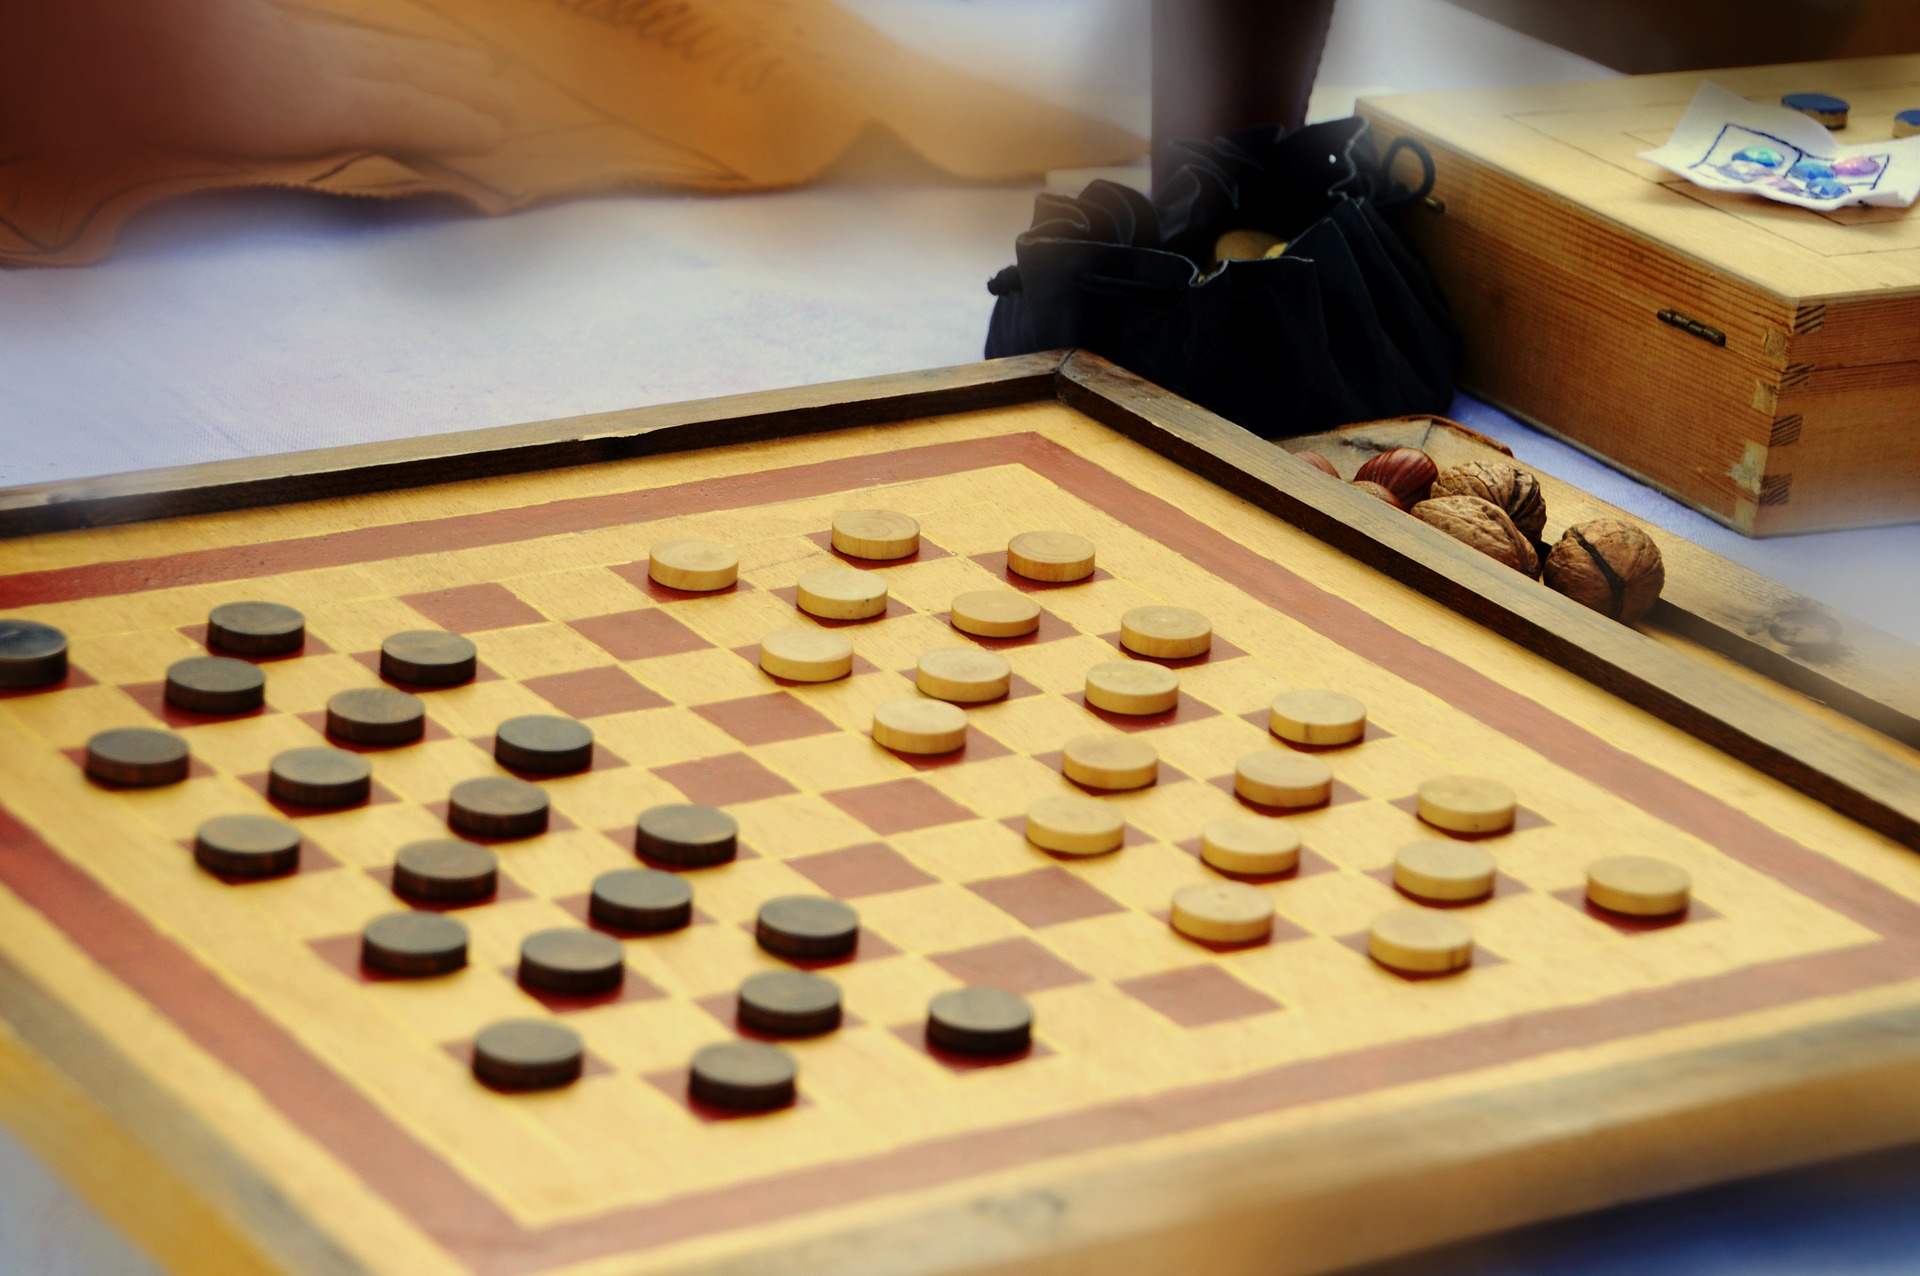
\includegraphics[scale=0.5]{img_dame.jpg}
  \end{center}
  
  \begin{center}
    Jeu de dame
  \end{center}

\end{frame}

\begin{frame}
  \frametitle{Introduction}

  \subsection{Règles de jeu}

  \begin{itemize}
    \item Le jeu se joue à 2 joueurs sur un plateau de taille n * n.
    \item Les joueurs jouent chacun à leur tour. Les blancs commencent toujours.
    \item Le but du jeu est de capturer tous les pions adverses. 
    \item Si un joueur ne peut plus bouger, même s'il lui reste des pions, il perd la partie. 
    \item Chaque pion peut se déplacer d'une case vers l'avant en diagonale. 
    \item Un pion arrivant sur la dernière rangée et s'y arrêtant est promu en « dame ».
    \item La dame se déplace sur une même diagonale d'autant de cases qu'elle le désire, en avant et en arrière.
  
  \end{itemize}

\end{frame}

\begin{frame}
  \frametitle{Introduction}
  \begin{itemize}
    \item Un pion peut en prendre un autre en sautant par dessus le pion adverse
     pour se rendre sur la case vide située derrière celui-ci. Le pion sauté est retiré du jeu.
    \item La prise est obligatoire.
    \item Lorsque plusieurs prises sont possibles, 
    il faut toujours prendre du côté du plus grand nombre de pièces.
    \item La dame doit prendre tout pion situé sur sa diagonale 
    (s'il y a une case libre derrière) et doit changer de direction à chaque 
    fois qu'une  nouvelle prise est possible. 
  \end{itemize}
\end{frame}

\begin{frame}
  \frametitle{Introduction}
\end{frame}

\begin{frame}
  \frametitle{Introduction}
\end{frame}
%
%
%%%%%%%%%%%%%%%%%%%%%%%%%%%%%%%%%%%%
\section{Bla bla bla}
%%%%%%%%%%%%%%%%%%%%%%%%%%%%%%%%%%%%
%
%
\begin{frame}
  \frametitle{Truc}
\end{frame}
%
%
\begin{frame}
  \frametitle{Machin}
\end{frame}
%
%
%%%%%%%%%%%%%%%%%%%%%%%%%%%%%%%%%%%%
\section{Conclusion}
%%%%%%%%%%%%%%%%%%%%%%%%%%%%%%%%%%%%
%
%
\begin{frame}
  \frametitle{Conclusion}
  \begin{itemize}
    \item
    \item
    \item
  \end{itemize}
\end{frame}
%
%
\end{document}
